% ============================================================================
% !Document: IG02 [zxweather Installation Reference]
% ----------------------------------------------------------------------------
% !Revision: 001
% !IssueDate: January 2013
% !Status: Unreleased
%
% !-Classification
% !ProjectCode: DAZW [Database Applications, zxweather]
% !Type: IG [Installation Guide]
%
% !Copyright: (C) David Goodwin, 2012, 2013
% !License: FDL [GNU Free Documentation License]
% !Auhtor: David Goodwin
% ============================================================================

% Document information. This should match the above
\newcommand{\doctitle}{zxweather}
\newcommand{\docsubtitle}{Installation Reference}
%\newcommand{\projectnum}{DAZW}
\newcommand{\docnum}{IG02}
\newcommand{\docrev}{001}
\newcommand{\docdate}{January 2013}
\newcommand{\docauthor}{David Goodwin}
\newcommand{\docabstract}{This manual provides installation and configuration guidelines for zxweather.}
\newcommand{\docupdateinfo}{This is a new manual}
\newcommand{\docosver}{Linux; Microsoft Windows NT 5.0+}
\newcommand{\docswver}{zxweather 0.2}
\newcommand{\doccopyright}{\textcircled{c} Copyright David Goodwin, 2012, 2013.}
\newcommand{\doclicense}{Use, reproduction and modification of this document is permitted subject to the terms of the GNU Free Documentation License, Version 1.3 or any later vesion published by the Free Software Foundation. See \url{http://www.gnu.org/copyleft/fdl.html} for full license text.}

%%%%%%%%%%%%%%%%%%%%%%%%%%%%%%%%%%%%%%%%%%%%%%%%%%%%%%%%%%%%%%%%%%%%%%%%%%%%%
%                                 CONFIGURATION                             %
%%%%%%%%%%%%%%%%%%%%%%%%%%%%%%%%%%%%%%%%%%%%%%%%%%%%%%%%%%%%%%%%%%%%%%%%%%%%%

% Book type document, A4 paper, 10pt std font size:
\documentclass[a4paper,10pt,draft]{book} 

\usepackage[scaled=0.90]{helvet} % Use helvetica as the standard font
\usepackage{courier}			 % Use courier as the fixed-width font
\usepackage{hyperref}			 % Links in PDF output
\usepackage{a4wide}				 % Narrower margins for A4 documents
\usepackage{ifthen}				 % A few if statements
\usepackage{multirow}			 % Column spanning in tables
\usepackage{graphicx}			 % For pictures
\usepackage{tabularx}			 % For customising table column types


% use zxtechdoc styles if they're there
\IfFileExists{zxtitle.sty}{\usepackage{zxtitle}}{}
\IfFileExists{zxtechdoc.sty}{\usepackage{zxtechdoc}}{}

\hypersetup{
    unicode=false,          % non-Latin characters in Acrobat’s bookmarks
    pdftoolbar=true,        % show Acrobat’s toolbar?
    pdfmenubar=true,        % show Acrobat’s menu?
    pdffitwindow=false,     % window fit to page when opened
    pdfstartview={FitH},    % fits the width of the page to the window
    pdftitle={\doctitle{} - \docsubtitle},    % title
    pdfauthor={\docauthor},     % author
    pdfsubject={\doctitle},   % subject of the document
    pdfkeywords={\doctitle} {\docsubtitle}, % list of keywords
    pdfnewwindow=true,      % links in new window
    colorlinks=true,       % false: boxed links; true: colored links
    linkcolor=black,          % color of internal links
    citecolor=green,        % color of links to bibliography
    filecolor=magenta,      % color of file links
    urlcolor=black           % color of external links
}

% Build the partnumber. Format is PROJ-DOCU.REV. If revision is 001 then it 
% is not displayed. If project is undefined it is not displayed.
\newcommand{\partnumber}{\ifthenelse{\isundefined{\projectnum}}{}{\projectnum-\docnum	\ifthenelse{\equal{\docrev}{001}}{}{.\docrev}}}

% ragged-right paragraphs for tabular environments. Use 'P' instead of 'p'.
\newcolumntype{P}[1]{>{\raggedright\arraybackslash}p{#1}}

\newcommand*\cleartoleftpage{%
  \clearpage
  \ifodd\value{page}\hbox{}\newpage\fi
}

\begin{document}

% Roman Numerals for the front matter
\pagenumbering{roman}

% Setup the titlepage. We will use the zxtitle format if its there,
% otherwise the much simpler standard LaTeX one.
\ifthenelse{\isundefined{\ordernumber}}{

% Standard LaTeX titlepage
\title{\doctitle{} - \docsubtitle}
\author{\docauthor}
}{

% zxtitle titlepage
\title{\doctitle}
\subtitle{\docsubtitle}
\titleabstract{\docabstract}
\ordernumber{\partnumber}
\updateinfo{\docupdateinfo}
\osinfo{\docosver}
\swversion{\docswver}
\titlecopyright{\doccopyright}
\licensestatement{\doclicense}
}
\date{\docdate}

\maketitle

\clearpage

\tableofcontents
\clearpage

%%%%%%%%%%%%%%%%%%%%%%%%%%%%%%%%%%%%%%%%%%%%%%%%%%%%%%%%%%%%%%%%%%%%%%%%%%%%%
%                                 DOCUMENT                                  %
%%%%%%%%%%%%%%%%%%%%%%%%%%%%%%%%%%%%%%%%%%%%%%%%%%%%%%%%%%%%%%%%%%%%%%%%%%%%%

%TODO : Normalise terminology across documents (use either 'sample' or 'history record').

\chapter{Introduction}
% Back to arabac numerals for the proper content
\pagenumbering{arabic}
\setcounter{page}{1}

zxweather a collection of tools to store and display data collected by automatic weather stations compatible with the Fine Offset WH1080. It is licensed under the GNU GPL making it free software.

Its main features are:
\begin{itemize}
\item A modern HTML5 web interface
\item Basic HTML fallback for older browsers
\item Full weather history
\end{itemize}

This manual provides installation and maintenance instructions for the entire core system. You should read this manual in its entirety to avoid problems.

This manual does \emph{not} cover an upgrade installation of zxweather v0.2. If you need to upgrade from a previous version consult the \emph{zxweather Upgrade Installation Guide, version 0.2} (\verb|DAZW-UR02|).

\begin {figure}[!ht]
 \centering
 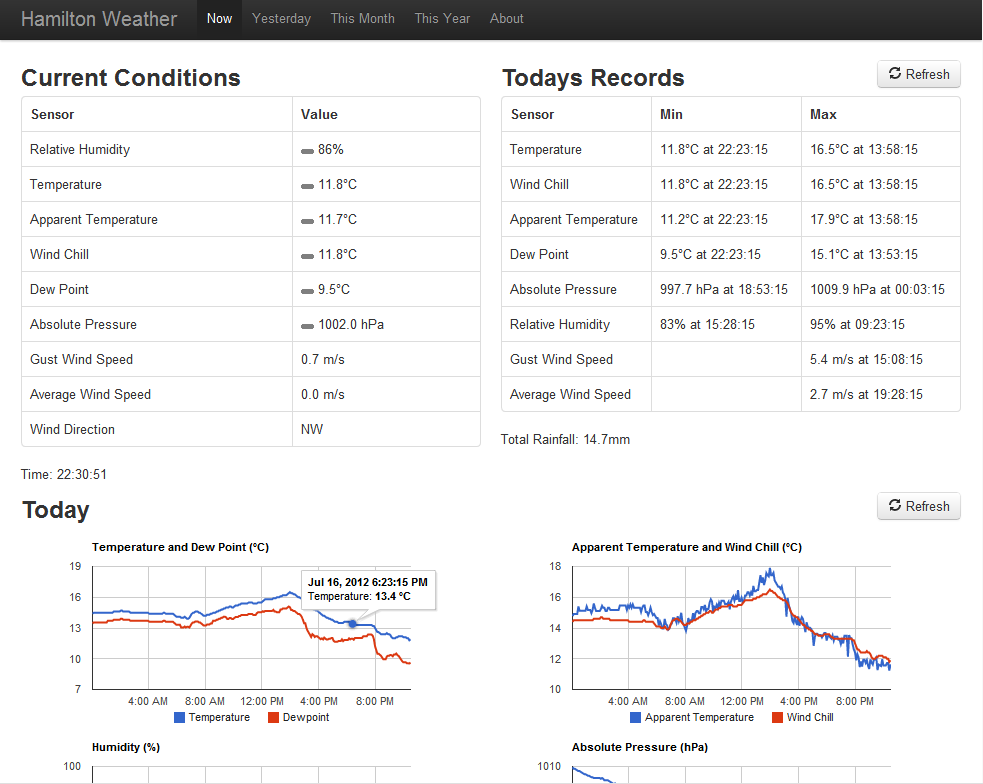
\includegraphics[scale=0.574]{images/stat_overview}
 \caption{Station Overview Page}
 \label{img_station_overview}
\end {figure}

\section{Related Documentation}
Other available documentation for the zxweather system include:

\begin{tabular}{l l}
\verb|DAZW-UR02| & zxweather Upgrade Installation Guide, version 0.2\\
\verb|DAZW-WG02| & WH1080 Utilities Users Guide, version 0.2 \\
\verb|DAZW-DB02| & zxweather Database Structure, version 0.2 \\
\end{tabular}

\section{System Structure}
zxweather consists of three major components:
\begin{itemize}
\item A PostgreSQL Database
\item Data Logger (wh1080d) and other WH1080 utilities
\item Web Interface
\end{itemize}

The database sits at the center of the zxweather system. The Data Logger feeds data into the database where the web interface and other clients can access it.

Because of this architecture all systems must be on the same network as the database server (using either SSH tunnels or VPNs). This can make running the Web Interface on a remote system (such as a VPS) difficult.

% TODO: Make a note about weather_push

\section{Supported Hardware}
This version of zxweather only supports weather stations 100\% compatible with the FineOffset WH1080. These weather stations are resold by many companies under various names.

The weather stations sample interval should be set to five minutes. If you have previously used software such as wview you may find your stations sample interval is set to one minute - this is not supported and will not work. Resetting your device should fix this.

Intervals larger than five minutes should work but there may be minor issues in the web interface.

\section{System Requirements}
Linux is strongly recommended as the operating system for running the core components of zxweather. 

While this manual does not cover installation or operation on systems running Microsoft Windows it is possible to do with some limitations if running under linux is not practical or possible.

The only supported database engine is PostgreSQL. Any version from 9.0 and up should be suitable. Older versions may work but this is not tested. Other RDBMS (such as MySQL) are not supported in any way.

The WH1080 tools are only supported on little-endian CPU architectures at this time. This includes Intel IA32 (x86) and most ARM processors. Bad things will happen if your processor is big-endian.

\subsection{Software Environment}
This section covers the software environment required to run the Data Logger and Web Interface. For PostgreSQL system requirements consult its documentation.

\subsubsection{Data Logger}

If you are running these tools under Microsoft Windows a binary distribution is available that contains all of the required libraries, etc. If you are using this then you do not need to read this section.

The Data Logger and other WH1080 utilities require the following libraries to be installed on your system:
\begin{itemize}
\item libusb-1.0 (on linux only)
\item libecpg (A part of ECPG)
\item libpq (PostgreSQL client library)
\end{itemize}

Additionally, to compile these you will need:
\begin{itemize}
\item GNU C Compiler and GNU Make
\item ECPG tool (a part of PostgreSQL)
\item Development packages for libusb-1.0 and libecpg
\end{itemize}

This software and libraries should be available from your operating systems package manager. On Debian 6.0 the packages would be \verb|build-essential| \verb|libusb-1.0-0-dev| \verb|libecpg-dev|.

\subsubsection{Web Interface}
The web interface requires the following to be installed on your system:
\begin{itemize}
\item Python 2.7
\item The following python libraries: 
\begin{itemize}
\item Psycopg2
\item web.py
\item Jinja2
\item python-gnupg
\end{itemize}
\item Gnuplot
\item Apache2 with mod\_wsgi (or another web server with WSGI support)
\end{itemize}

\section{Distribution Contents}
The standard zxweather distribution should be extracted to somewhere on your disk such as \\ \verb|/opt/zxweather|:

\begin{verbatim}
$ pwd
/opt/zxweather
$ ls
admin_tool  database  desktop  doc  plot  wh1080  zxw_web
\end{verbatim}

The subdirectories are:

\begin{itemize}
\item \emph{admin\_tool} - Tool for creating and upgrading databases
\item \emph{database} - Scripts to create the database (chapter \ref{cha_database})
\item \emph{desktop}  - Desktop interface
\item \emph{doc} - Documentation
\item \emph{plot} - Tools for plotting static charts (chapter \ref{cha_web_interface})
\item \emph{wh1080} - The Data Logger and other WH1080 utilities (chapter \ref{cha_data_logger})
\item \emph{zxw\_web} - The web interface (chapter \ref{cha_web_interface})
\end{itemize}

The wh1080 and desktop directories contain C/C++ source code. If you are running Microsoft Windows pre-compiled versions of these programs are available. See \url{http://ftp2.zx.net.nz/pub/DGS/zxweather/readme.html} for download links.

The doc directory contains \LaTeX{} source code for producing the zxweather documentation as well as the compiled versions in Adobe PDF format. This documentation is available in other formats from the URL above.

\chapter{Database}
\label{cha_database}
% Instructions for how to setup the database. This includes permissions
% required, etc.

This chapter describes the database setup required by zxweather. The database is required by the core system and is not optional. It must be setup on a system that all other components have network access to.


%Alternatively, if it is impractical for all systems to have direct access to the database it is possible to setup a second replica database on the system running the Web Interface. Chapter \ref{cha_db_replication} covers this setup in more detail.

If you already have a database from a previous installation of zxweather v0.2 that you wish to re-use you can skip this chapter. If you already have a database but it is from a previous installation of zxweather v0.1.x then the database will need upgrading. This is covered by chapter 3 of the \emph{zxweather Upgrade Guide, version 0.2} (DAZW-UR02).

\section{Installation}
The zxweather database has only been tested with PostgreSQL version 9.0 and above. This documentation assumes you already have a suitable version of the server and client tools installed on your system.

This section documents creating the zxweather database using the command-line admin tool. If you would rather create the database yourself the create script is called \verb|database.sql| and can be found inside the database subdirectory of the zxweather distribution. 


\subsection{Create Database}
To start the admin tool execute \verb|python admin_tool/admin_tool.py| in the zxweather distribution directory:

\begin{verbatim}
$ pwd
/opt/zxweather
$ ls
admin_tool  database  desktop  doc  plot  wh1080  zxw_web
$ python admin_tool/admin_tool.py
\end{verbatim}

When you start it you will be given a list of options for connecting to a database:
\begin{verbatim}
ZXWeather v0.2 admin tool
        (C) Copyright David Goodwin, 2013

Select option:
        1. Create a new weather database
        2. Connect to an existing weather database
        0. Exit
Choice>
\end{verbatim}

To create a new database enter 1 and hit return. You will then be asked for details about your database server. You will need:
\begin{itemize}
\item hostname or IP address
\item port (this is normally 5432)
\item username
\item password
\end{itemize}
You should login as a user with database creation permissions such as the postgres user.

\subsubsection{Hostname}
The first question you will be asked is for the hostname of the database server:
\begin{verbatim}
Enter the details for the database you wish to create
You will now be prompted for database configuration details.
Hostname [localhost]:
\end{verbatim}

If the database server is running on the same machine you are running the admin tool on you can simply hit return to accept the default value shown in square brackets (localhost).

\subsubsection{Port}
The second question is the database servers port number:
\begin{verbatim}
Port [5432]:
\end{verbatim}
You should be able to just hit return here unless you or someone else has changed PostgreSQL to run on a port other than the default of 5432.

\subsubsection{Database name}
Next you will be asked for the name of the new database. This must be a valid PostgreSQL identifier. It must start with a letter and can contain only letters, digits or the underscore character as described below:

\begin{verbatim}
The database name must start with a letter and may only contain 
letters, digits or the underscore character ('_'). Valid database
names include weather, weather42, my_weather_database, 
weather_42_database. If your database name does not meet these 
restrictions you'll get an error later on.
New database name [weather]:
\end{verbatim}

Again, if you are happy with your database being called "weather" you can just hit return.

\subsubsection{Username and password}
Lastly you will be asked for the username and password of a user who has enough rights to create new databases. The new database will be owned by this user. It is recommended you use the standard PostgreSQL administrator account "postgres":
\begin{verbatim}
Username [postgres]:
Password:
\end{verbatim}

Once you have entered a username and password your new database will be created. The output of this process should look something like the following if your database was successfully created:
\begin{verbatim}
Connect succeeded. Server version: PostgreSQL 9.2.0, 64-bit
Loading create script...
Creating new database...
Reconnect succeeded. Server version: PostgreSQL 9.2.0, 64-bit
Creating database structure. This may take a little while...
New database created successfully.
Connect succeeded. Server version: PostgreSQL 9.2.0, 64-bit
\end{verbatim}

\subsubsection{Creating a station}

You should now at the normal administration menu shown below:
\begin{verbatim}
Select option:
        1. Manage stations
        2. Upgrade about.html
        0. Exit
Choice>
\end{verbatim}

You must now create a new weather station in the database by selecting option 1 from the menu (enter 1 and hit enter). This will take you to the Manage Stations menu:

\begin{verbatim}
Manage Stations
---------------

Select option:
        1. List stations
        2. Create station
        3. Edit station
        0. Return
Choice>
\end{verbatim}

Select option 2 from the list to create a new station. You will be asked for the following details about your station:
\begin{itemize}
\item Station Code
\item Station Name
\item Description
\item Hardware Type
\item Sample Interval
\item If live data is available from the station
\end{itemize}

\subsubsection{Station Code}
The station code is a short (maximum of 5 characters) unique code to identify your weather station. It can not be changed later.

\begin{verbatim}
              |---|
Station Code:
\end{verbatim}

The prompt includes a bar above it to show you how long the station code is allowed to be.

\subsubsection{Station Name and Description}
The station name is a short name for your weather station. The description field allows you to enter a longer description of your weather station. Both of these can be changed later by selecting the "Edit station" option from the "Manage Stations" menu.

\begin{verbatim}
Station Name is a longer name for your station that will be displayed 
to users.
Name: Test station

You may now enter an optional short description for your weather
station.
Description []:
\end{verbatim}

The description is optional so you can just hit return if you don't want to enter one.

\subsubsection{Hardware Type}
Next you must specify what sort of weather station hardware you will be using. As shown below this version of zxweather only supports one type of weather station - the Fine Offset WH1080. As such \verb|FOWH1080| is your only option so enter that exact code in response to the question.

\begin{verbatim}
Code     Title
-------- ----------------------------------------------------------
FOWH1080 Fine Offset WH1080-compatible
-------- ----------------------------------------------------------
Hardware type code:
\end{verbatim}

\subsubsection{Sample Interval and Live Data}

The final two questions are asking you about what sort of data is available from your weather station.

The sample interval is how often your weather station records new samples. Five minutes (300 seconds) is the recommended number. Values less than this are not supported and will not work. If you have previously used wview with your weather station you may find it is set to 60 seconds. Resetting your weather station console should fix this. Alternatively you can use the EasyWeather software that came with your weather station to manage the sample interval.

You should answer yes to the following question about live data. Should you decide not to use wh1080d as your data logger you can come back to the station management menu later to turn this option off.

\begin{verbatim}
The stations sample interval is how often new samples are loaded 
into the database. Samples are used to plot charts and are also 
used for the current conditions when live data is not available. 
The sample interval is in seconds where 300 is 5 minutes.
Sample interval [300]:
Is live data available for this station (yes/no) [yes]:
\end{verbatim}

\subsubsection{Finishing Up}
You have now finished entering all data required for your weather station. You will finally be asked to confirm the details you have entered. This is your opportunity to correct any typos, etc.

\begin{verbatim}
You entered the following details:
----------------------------------
Code: rua
Name: Ruakura Station
Sample interval: 300
Live data available: True
Hardware type: FOWH1080
Description:

----------------------------------

If you no longer wish to create this station answer no to the 
following two questions.

Is the information entered correct? (y/n):
\end{verbatim}

Answering 'y' here will create the station. Remember that stations can not be removed so if you do not wish to create the station you should answer 'n' here.

Answering 'n' will give you the option to either cancel or adjust your answers.

\section{Permissions}
If you wish to create separate user accounts for zxweather then the various programs need the following permissions listed below. Creating new PostgreSQL user accounts is not covered by this manual.

\begin{tabular}{l l}
\hline
\textbf{Program} & \textbf{Permissions} \\
\hline
wh1080d & CONNECT, SELECT, INSERT, UPDATE \\
wh1080 & CONNECT, SELECT, INSERT \\
weatherplot & CONNECT, SELECT \\
web interface & CONNECT, SELECT \\
\hline
\end{tabular}

%\subsection{Creating Accounts}
%TODO Instructions for creating the accounts

\chapter{Data Logger}
\label{cha_data_logger}
% Compiling and installing wh1080d or the other program

The Data Logger is a daemon which continuously downloads weather data (both live and historical samples) from the weather station and loads it into the database. It is called \emph{wh1080d} and is one of the WH1080 Utilities. Its full documentation is contained in the \emph{WH1080 Utilities Users Guide, version 0.2} (DAZW-WG02).

This chapter covers how to compile and install this tool. Additionally, section \ref{sec_loading_data} includes some important maintenance information that must always be taken into consideration before you start wh1080d.

\section{Compiling}
This section only covers compiling the tools under Linux. If you are using Microsoft Windows it is recommended that you use the pre-compiled executables and skip to the next section.

\subsection{Requirements}
To compile the tools under Linux the following software must be installed:
\begin{itemize}
\item GNU Make
\item GNU C Compiler
\item ECPG (a PostgreSQL utility)
\end{itemize}

The following development libraries are also required:
\begin{itemize}
\item libpq (PostgreSQL client library)
\item libecpg (library for ECPG)
\item libusb-1.0
\end{itemize}

These libraries and software packages should be available from your operating systems package manager. On Debian 6.0 the packages would be \verb|build-essential libusb-1.0-0-dev libecpg-dev|.

\subsection{Compiling the WH1080 Tools}

%TODO Switch to the GNU Build System and rewrite this.

To compile the WH1080 tools, cd into the wh1080 subdirectory of the zxweather distribution and run \verb|make|. This should kick off the build process and leave you with a handful of programs inside the wh1080 directory.

\section{Loading Data}
\label{sec_loading_data}

Before you can start the data logger on a non-empty database it is important to note that you may have to run a \emph{full update} using the \emph{wh1080 tool} first. This prevents existing data stored in your weather stations memory from being lost.

Performing a full update when it is not necessary will result in duplicate data being loaded into your database. It is important that a full update is performed only when necessary.

\subsection{When to perform a Full Update}
There are only three occasions when it is acceptable to perform a full update:
\begin{itemize}
\item You have just erased the weather stations memory
\item You have reset the weather station
\item The database is more than 4080 samples out of date
\end{itemize}

The first two deal with the case where the sample the database says needs to be downloaded next no longer exists on the weather station. The data logger will detect this condition and will refuse to start printing out the message below:
\begin{verbatim}
Checking for station reset condition...
Fatal Error: wh1080d cannot be restarted after a device reset. Consult 
installation reference manual for maintenance procedure to clear error
condition.
\end{verbatim}

Performing a full update will fix this and allow the data logger to start.

The third occasion when it is acceptable to perform a full update is when your database is very out of date such that no sample on the weather station exists in your database. This condition is not detected automatically.

In this case it is not strictly necessary to perform a full update as failure to do so will not cause any damage. Not performing a full update in this case will just result in some new data on your weather station being missed.

In order for a full update to be necessary your weather station must be more than 4080 samples out of date. If it is configured to take one sample every five minutes then the database must be more than 340 hours out of date (a little over 14 days).

If in any doubt perform a full update on a test database and compare what it download with what is already in your weather database to see if there is any overlap at all.

\subsection{Performing a Full Update}
To perform a full update you must use the the wh1080 tool as the data logger (wh1080d) can not perform this operation. wh1080 is one of the WH1080 Utilities and is a basic tool for inspecting the contents of the weather station and downloading samples into a database.

The \verb|-l| command-line option causes the wh1080 tool to perform a Full Update instead of a regular one:

\verb|wh1080 -l -d databasename@hostname -u username -p password -s code|

This is covered in more detail in Section 2.2.4 of \emph{WH1080 Utilities Users Guide} (DAZW-WG02).

\section{wh1080d Configuration}
\subsection{Linux}

wh1080d (the Data Logger) takes the following arguments:

\begin{tabular}{l l p{10cm}}
\hline
\textbf{Argument} & \textbf{Parameter} & \textbf{Description} \\
\hline
-d & database & Database connection string \\
-u & username & Database username \\
-p & password & Database password \\
-s & station  & Station Code for weather station to work against \\
-f & filename & Log file to write messages to \\
\hline
\end{tabular}

Under linux the Update Service runs as a daemon. To start it just run something like the following from your system startup scripts:

\verb|wh1080d -d database -u username -p password -s rua -f logfile|

The log file is truncated when the daemon starts.

\subsection{Windows}

%TODO Add the ability to run wh1080d as a windows service and document it here.

Currently wh1080d is not capable of running as a service on windows. Instead you must run the wh1080dtest program which provides the same functionality but stays open in a console window. It takes the following arguments:

\begin{tabular}{l l p{10cm}}
\hline
\textbf{Argument} & \textbf{Parameter} & \textbf{Description} \\
\hline
-d & database & Database connection string \\
-u & username & Database username \\
-p & password & Database password \\
-s & station  & Station Code for weather station to work against \\
\hline
\end{tabular}

This may change in a future release.

\chapter{Web Interface}
\label{cha_web_interface}

The Web Interface is the primary way for viewing data in the zxweather database. It consists of two components - the WSGI web application and the chart plotting program.

Both components are required for correct operation. This chapter describes how to install and configure them.

% Overview of features

\section{WSGI Application}

The web interface is written as a Python WSGI application. This section only covers installing the application under Apache httpd. If you are not using Apache then consult your web servers documentation for instructions on installing wsgi applications.

\subsection{Installation}
% Where to put it
% Apache configuration

At this time zxweather cannot be run in a subdirectory - it must live in the root directory of the website. This generally means giving it its own virtual host.

The system you are installing the web interface on must have the following installed on it:
\begin{itemize}
\item Apache httpd
\item mod\_wsgi
\item Python 2.6 or 2.7 with the following packages:
\begin{itemize}
\item psycopg2
\item web.py
\item python-gnupg
\end{itemize}
\end{itemize}

Installation and configuration of these packages is outside the scope of this document. If you are setting up on a Linux system the packages are likely all available from your distributions package repositories. 

Where examples are provided in this section they are for Debian-based Linux distributions. Installation and configuration on Windows systems is similar but requires more effort.

\subsubsection{WSGI Setup}
As the zxweather web interface is a Python WSGI application you must have the mod\_wsgi installed and enabled. On Debain-based systems the package is called \verb|libapache2-mod-wsgi| and can be enabled using the \verb|a2enmod| tool:

\begin{verbatim}
$ a2enmod wsgi
\end{verbatim}

\subsubsection{Virtual-host Configuration}

All that is required to make zxweather work from the Apache end is adding the following to your vhost configuration file:
\begin{verbatim}
WSGIScriptAlias / /opt/zxweather/zxw_web/zxweather.py
\end{verbatim}

An example virtual host configuration might look like this:

\begin{verbatim}
<VirtualHost *:80>
        ServerAdmin admin@example.com
        ServerName weather.example.com

        DocumentRoot /var/www
        ErrorLog ${APACHE_LOG_DIR}/weather-error.log
        LogLevel warn
        CustomLog ${APACHE_LOG_DIR}/weather-access.log combined

        WSGIScriptAlias / /opt/zxweather/zxw_web/zxweather.py
</VirtualHost>
\end{verbatim}

\subsection{Configuration}
% The configuration file

The Web Interface attempts to load configuration files in the following order. Only the first one it finds is loaded.
\begin{itemize}
\item \verb|config.cfg| (in the current directory)
\item \verb|zxw_web/config.cfg|
\item \verb|/etc/zxweather.cfg|
\end{itemize}

It is recommended that you install your configuration file in \verb|/etc|. To do this, copy the \\ \verb|zxweather.cfg.sample| file included in the zxweather distributions \verb|zxw_web| subdirectory:
\begin{verbatim}
$ cp /opt/zxweather/zxw_web/zxweather.cfg.sample /etc/zxweather.cfg
\end{verbatim}

This configuration files format is similar to the INI format commonly used on Microsoft Windows. The '\#' character marks a comment, group names are inside square brackets. Key-value pairs are written in the following way:
\begin{verbatim}
key: value
\end{verbatim}

\subsubsection{Database}
The first group is for database configuration. It looks like the following:
\begin{verbatim}
[database]
host: localhost
port: 5432
database: weather
user: weatheruser
password: password
\end{verbatim}

Where the settings are:
\begin{itemize}
\item host - the hostname or IP address of your database server
\item port - The port your database listens on. This is commonly 5432 for PostgreSQL
\item database - Name of your database
\item user - The user to login to the server as
\item password - The users password
\end{itemize}


\subsubsection{Site}
The Site group stores basic web interface configuration:
\begin{verbatim}
[site]
default_ui: s
site_name: zxweather
# UNCOMMENT THESE AND SET THEM! The defaults will NOT work.
#site_root: http://weather.example.com/
#static_data_dir: /opt/zxweather/zxw_web/weather/static/
#station_name: abc
\end{verbatim}

Where the settings are:
\begin{itemize}
\item default\_ui - The default UI to use. 's' is the Standard UI, 'b' is the Basic (HTML-only) UI. Unless your only browser is from 2001 you will want to leave this on 's'.
\item site\_name - The name of your site. This appears on the left of the navigation bar and in the title of every page.
\item site\_root - The URL for the root of your website. For example, http://weather.example.com/.
\item static\_data\_dir - Where on your hard disk the static data directory is. If zxweather was extrated to \verb|/opt/zxweather| then this should be set to \verb|/opt/zxweather/zxw_web/static/|.
\end{itemize}

The final setting in this group is station\_name. This is the default weather station to show data for when a user first arrives at your site. It should match the station code you chose when creating your database.

You must also create a directory of the same name inside the static data directory. If your weather station code is "foo" then you would:
\begin{verbatim}
$ mkdir /opt/zxweather/zxw_web/static/foo
\end{verbatim}

\subsection{About Page}
% About page
On the navigation bar of the standard Web Interface is an "About" link which will take you to a generic about page which you will want to customise.

To do this, navigate into the \emph{static data} directory ( \verb|/zxw_web/static/|) and copy the \verb|about.html| file into your weather stations subdirectory. If, for example, your station is called "foo" and zxweather is installed in \verb|/opt/zxweather| you would copy \verb|/opt/zxweather/zxw_web/static/about.html| to \\ \verb|/opt/zxweather/zxw_web/static/foo/about.html|. You can then customise this copy of the file. You should avoid modifying the original copy as it may be overwritten without warning by future versions.

When editing your copy of \verb|about.html| you will find two comments near the bottom of the page; \\
\verb|<!-- BEGIN_USER_CONTENT -->| and \verb|<!-- END_USER_CONTENT -->|. You can put anything you want between these comments.

It is best to avoid making any changes outside of these comments as future versions may make changes to the file outside these comments as part of the upgrade process.


\section{Chart Plotting}
\label{sec_chart_plotting}
% Purpose of this program
% Command-line arguments
% How to set it up

The \emph{weatherplot} program is responsible for generating static charts primarily used by the basic HTML web interface. It must be setup as a scheduled task to be run at regular intervals.

The machine it runs on must have \emph{gnuplot} installed and must have access to the database server and directory the zxweather web interface runs from.

\subsection{Usage}

The weatherplot program is written in the Python language and lives in the \verb|plot| subdirectory of the zxweather distribution. It is executed on the command-line with python as: \\ \verb|$ python plot/weatherplot.py [arguments]|.

The charts it generates must be put in the web interfaces \emph{static data} directory in a subdirectory with the same name as your station. For example, if your station is named "foo" and the zxweather distribution was extracted to \verb|/opt/zxweather| then you would generate charts into \\ \verb|/opt/zxweather/zxw_web/static/foo/|.

By default an executable called \verb|gnuplot| is expected to be in the path which it can use to generate the charts. If your install of gnuplot is not in the path or goes by another name use the \verb|--gnuplot-binary| parameter to specify its name.

\subsubsection{Command-line Arguments}
The weatherplot program accepts the following command-line arguments:

\begin{tabular}{p{3.4cm} l p{8cm}}
\hline
\textbf{Argument} & \textbf{Parameter} & \textbf{Description} \\
\hline
\verb|-t| \par \verb|--database| & dbname & Name of the database to use. Required. \\
\verb|-n| \par \verb|--host| & hostname & Database server hostname. Required. \\
\verb|-u| \par \verb|--user| & username & Username for database server. Required. \\
\verb|-p| \par \verb|--password| & password & Password for database server. Required. \\
\verb|-d| \par \verb|--directory| & directory & Output directory. Required. \\
\verb|-a| \par \verb|--plot-new| & filename & Only plots charts for dates on or after that stored in the specified file. \\
\verb|-r| \par \verb|--replot-pause| & seconds & Number of seconds to wait before replotting.\\
\verb|-g| \par \verb|--gnuplot-binary| & filename & Name of the gnuplot executable to use if it is something other than "gnuplot".\\
\verb|-s| \par \verb|--station| & code & The station code of the weather station to plot charts for.\\
\hline
\end{tabular}

The database, host, user, password, directory and station parameters are always required.

\subsection{Plotting All Charts}

To regenerate charts for your entire database run the weatherplot program with only the minimum command-line arguments:

\begin{verbatim}
$ python plot/weatherplot.py --database weather --host localhost \
--user postgres --password password \
--directory zxw_web/static/station_name/
--station station_code
\end{verbatim}

This will create charts for all days and months in your database and store them in the specified directory. Depending on the size of your database this may take some time.

Some software upgrades may require you to do this when new chart types have been added or the style of the charts has been adjusted.

\subsection{Running as a Scheduled Task}

The recommended way to setup the weatherplot program is to run it as a scheduled task from cron or the windows task scheduler. When run in this way it is important that it be set to only plot charts containing new data.

The \verb|--plot-new| command-line argument implements this. The argument takes a single parameter which is the name of a file to store the date of the last plotted day in.

Each time the weatherplot program is executed with this parameter it will replot all charts for all days and months on or after the date in that file and then update the file with todays date. That way only charts that need to be regenerated are regenerated.

\subsubsection{Example}

When run as below weatherplot will only replot charts that have changed since it was last run:
\begin{verbatim}
$ python plot/weatherplot.py --database weather --host localhost
--user postgres --password password --directory static/station_name/
--plot-new plot_status_file --station station_code
\end{verbatim}

To make this run every 30 minutes you would add a line such as the following to /etc/crontab:
\begin{verbatim}
0,30 *  * * *   root    cd /opt/zxweather && \
  python plot/weatherplot.py -t weather -n localhost -u postgres \
  -p password -d zxw_web/static/station_name -a plot_status_file \
  -s station_code
\end{verbatim}

If the static charts are not important to you, you may wish to only regenerate them every few hours or once a day.

\subsection{Plotting Continuously}

The weatherplot program is capable of running interactively in continuous mode. When run like this it will automatically replot charts at a specific interval until you terminate it with Ctrl+C. This is primarily intended for testing purposes.

It can be run in this mode by supplying the \verb|--replot-pause| parameter
with a suitable interval in seconds.

\subsubsection{Example}

When run as below the behaviour is the same as setting it up to be run by cron every 30 minutes except it runs continuously attached to the terminal.

\begin{verbatim}
$ python plot/weatherplot.py --database weather --host localhost \
--user postgres --password password --directory zxw_web/static/rua \
--plot-new plot_status_file --replot-pause 1800 --station rua

Weather data plotting application v1.1
        (C) Copyright David Goodwin, 2012, 2013


Connecting to database...
Server version: PostgreSQL 9.2
Generating temperature plots in zxw_web/static/rua
Plotting from 2012-05-10
Plotting graphs for 2012...
Plotting graphs for 2012 may...
Plot zxw_web/static/rua/2012/may/temperature_tdp_large.png
Plot zxw_web/static/rua/2012/may/temperature_awc_large.png
Plot zxw_web/static/rua/2012/may/humidity_large.png
Plot zxw_web/static/rua/2012/may/indoor_humidity_large.png
Plot zxw_web/static/rua/2012/may/pressure_large.png
Plot zxw_web/static/rua/2012/may/indoor_temperature_large.png
Plot zxw_web/static/rua/2012/may/temperature_tdp.png
Plot zxw_web/static/rua/2012/may/temperature_awc.png
Plot zxw_web/static/rua/2012/may/humidity.png
Plot zxw_web/static/rua/2012/may/indoor_humidity.png
Plot zxw_web/static/rua/2012/may/pressure.png
Plot zxw_web/static/rua/2012/may/indoor_temperature.png
Plotting graphs for 2012 may 9...Skip
Plotting graphs for 2012 may 10...
Plot zxw_web/static/rua/2012/may/10/temperature_tdp_large.png
Plot zxw_web/static/rua/2012/may/10/temperature_awc_large.png
Plot zxw_web/static/rua/2012/may/10/humidity_large.png
Plot zxw_web/static/rua/2012/may/10/indoor_humidity_large.png
Plot zxw_web/static/rua/2012/may/10/pressure_large.png
Plot zxw_web/static/rua/2012/may/10/indoor_temperature_large.png
Plot zxw_web/static/rua/2012/may/10/temperature_tdp.png
Plot zxw_web/static/rua/2012/may/10/temperature_awc.png
Plot zxw_web/static/rua/2012/may/10/humidity.png
Plot zxw_web/static/rua/2012/may/10/indoor_humidity.png
Plot zxw_web/static/rua/2012/may/10/pressure.png
Plot zxw_web/static/rua/2012/may/10/indoor_temperature.png
Plot zxw_web/static/rua/2012/may/10/7-day_temperature_tdp_large.png
Plot zxw_web/static/rua/2012/may/10/7-day_temperature_awc_large.png
Plot zxw_web/static/rua/2012/may/10/7-day_humidity_large.png
Plot zxw_web/static/rua/2012/may/10/7-day_indoor_humidity_large.png
Plot zxw_web/static/rua/2012/may/10/7-day_pressure_large.png
Plot zxw_web/static/rua/2012/may/10/7-day_indoor_temperature_large.png
Plot zxw_web/static/rua/2012/may/10/7-day_temperature_tdp.png
Plot zxw_web/static/rua/2012/may/10/7-day_temperature_awc.png
Plot zxw_web/static/rua/2012/may/10/7-day_humidity.png
Plot zxw_web/static/rua/2012/may/10/7-day_indoor_humidity.png
Plot zxw_web/static/rua/2012/may/10/7-day_pressure.png
Plot zxw_web/static/rua/2012/may/10/7-day_indoor_temperature.png
Plot completed at 2012-05-10 22:31:46.953000
Waiting for 1800 seconds to plot again. Press Ctrl+C to terminate.
\end{verbatim}

\chapter{Troubleshooting}

\section{Data Logger}

\begin{tabular}{P{4.5cm} P{4.5cm} P{4.5cm}}
\hline
\textbf{Problem} & \textbf{Cause} & \textbf{Solution} \\
\hline
The data logger has crashed trying to read from the weather station. & The weather station has crashed (the history function on the weather station console does not work) & Kill the data logger process, hard-reset the weather station (remove and reinstall batteries and USB cable) and then restart the data logger after performing a full update. \\[0.2cm]
\multirow{6}{*}{\parbox{4.4cm}{The data logger exits with a database error written to the log file}} & The connection to the database was lost & Check database connectivity and restart the data logger. \\[0.2cm]
& Database parameters are incorrect & Check database parameters and restart the data logger. \\[0.2cm]
& The database was not created correctly. & Recreate the database and restart the data logger. \\
\hline
\end{tabular}

\section{Web Interface}
This section covers errors you may encounter when viewing pages in the web interface.

\begin{tabular}{P{4.5cm} P{4.5cm} P{4.5cm}}
\hline
\textbf{Problem} & \textbf{Cause} & \textbf{Solution} \\
\hline
The station overview page gives a "404 Not Found" error & The database is empty & Wait for data to appear in the database \\
\hline
\end{tabular}

% 

%%%%%%%%%%%%%%%%%%%%%%%%%%%%%%%%%%%%%%%%%%%%%%%%%%%%%%%%%%%%%%%%%%%%%%%%%%%%%
%                                END DOCUMENT                               %
%%%%%%%%%%%%%%%%%%%%%%%%%%%%%%%%%%%%%%%%%%%%%%%%%%%%%%%%%%%%%%%%%%%%%%%%%%%%%

% Back page
\cleartoleftpage
\thispagestyle{empty}
\begin{flushright}
\null
\vfill
\tt \partnumber
\end{flushright}
\end{document}